\section{Geometric interpretation of random variables}\label{rvs}

It is fundamental to define the geometric properties of random
variables using linear algebra.

Consider the vector space which consists of all random variables with finite
mean and variance.
We will regard each point in this space (or vector that correponds to that point
in terms of linear algebra) as a random variable.
We define the scalar product of two random variables $X$ and $Y$ to be
\[
\langle X, Y \rangle = \Cov(X,Y).
\]
It is not difficult to check that the definition satisfies the properties
of a scalar product assuming that $X$ and $Y$ are the same random variables
if $\P(X=Y)=1$.

\begin{marginfigure}
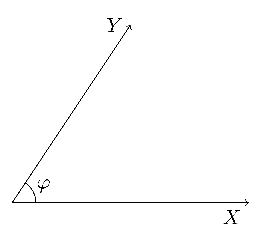
\includegraphics{figures/01_corr_def.pdf}
\caption{Geometric representation of random variables.}
\label{fig:corr_def}
\end{marginfigure}

Having defined the scalar product, we are now able to introduce the squared
length of a random variable $X$ which is
\[
\lVert X \rVert^2 = \langle X, X \rangle = \Cov(X,X) = \Var(X),
\]
so the~standard
deviation of $X$ ($\sigma_X$) is the length.

Recall that for any non-random vectors $a$ and $b$ the angle
between them is calculated with the formula
\[
\cos(a, b) = \frac{\langle a,  a\rangle}{|a| |b|}.
\]
The same applies for the random variables and it is already clear that
two random variables are uncorrelated iff their scalar product
equals $0$. Additionally, it means that these two random variables
are orthogonal in the vector space.

The analogue for $\cos(a, b)$ in the vector space of all the random
variables is the correlation between two of them:
\[
\Corr(X,Y) = \frac{\Cov(X,Y)}{\sqrt{\Var(X)\Var(Y)}} = \frac{\langle X, Y \rangle}{\sqrt{\lVert X \rVert^2 \lVert Y \rVert^2}}.
\]
From the equivalence of $\Corr(X,Y)$ to $\cos(a, b)$ it
automatically follows that the correlation coefficient can range from $-1$ to $1$.

% proofreaded up to this line

\begin{marginfigure}[10\baselineskip]
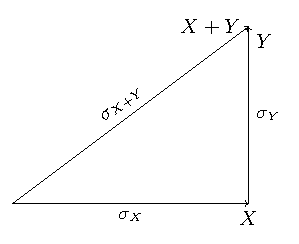
\includegraphics{figures/01_pythagorean_theorem.pdf}
\caption{The Pythagorean theorem for random variables $X$ and $Y$.}
\label{fig:rv_pyth}
\end{marginfigure}

A useful property of the geoemtry of random variables is that all the
geometric theorems still hold. For instance, the Pythagorean theorem can
be formulated as follows: if the ranadom variables $X$ and $Y$ are uncorrelated
(which implies that they are orthogonal), then the variance of their sum equals
the sum of their variances:
\[
\Var(X + Y) = \sigma^2_{X+Y} = \sigma^2_{X} + \sigma^2_{Y} = \Var(X) + \Var(Y).
\]
Translated to the non-random language, assumption of uncorrelatedness correspnds
to the right triangle setting, the variance of the sum of two random variables
stands for the hypotenuse squared and the sum of the variances is the sum of
the legs squared.

Another important geometric tool is projection.
Recall that for any two vectors the scalar product $\langle a, b \rangle$
can be interpreted as the length of projected $b$ multiplied by the length of $a$.
The projection itself is $\cos(a, b) b$.
Same holds for the random variables.
The projection of such a random variable $Y$ onto $\{cX| c \in \mathbb{R}\}$ is
$\hat Y = \Corr(X,Y) \cdot Y$.

\begin{marginfigure}
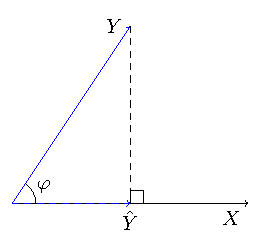
\includegraphics{figures/01_basic_projection.pdf}
\caption{The projection of a random variable $Y$ onto the line spanned by
a random variable $X$.}
\label{fig:rv_proj}
\end{marginfigure}

Note that the squared lengths of the leg adjacent to $\varphi$ and the
hypotenuse are $\Var(\hat Y)$ and $\Var(Y)$.
So, the Figure~\ref{fig:rv_proj} gives a useful expression for the correlation
coefficient squared:
\[
\Corr^2(X,Y) = \frac{\Var(\hat Y)}{\Var(Y)}.
\]

\subsection{The law of iterated expectations}

\marginnote{
Here is the proof for the case when $X$ and $Y$ are both discrete. Let $\E(Y|X) = g(X)$.
\begin{align*}
&\E(g(X)) = \sum_x g(x) \P(X=x) \\
&= \sum_x \left( \sum_y y \P(Y=y|X=x) \right) \P(X=x) \\
&= \sum_x \sum_y y  \P(X=x) \P(Y=y|X=x)  \\
&= \sum_y y \sum_x \P(X=x, Y=y) \\
&= \sum_y y \P(Y=y) = \E(Y)
\end{align*}
The proof in case of continous random variables is absolutely analogous.
}

\begin{theorem}
For any random variable $X$ and $Y$,
\[
\E(\E(X|Y)) = \E(Y).
\]
\end{theorem}

\begin{proof}

Consider a vector space of all the random variables.  The random variables
which can be described as functions of $X$ form a subspace of that vector
space, represented as a plane $\alpha$ in Figure~\ref{fig:adams}.
Another subspace is a subspace of constants, denoted as a vector $\mathbf{1} \in \alpha$.

In order to obtain $\E(Y|X)$, first, we need to project $Y$ onto the subspace
of all the functions of $X$. As a result of this step, we get $\E(Y|X)$ — the function
of $X$ that predicts $Y$ the best (the function which gives the lowest MSE).
Next, projecting $\E(Y|X)$ onto the space of all constants, we obtain $E(Y)$.

Notice that the vector $Y - \E(Y|X)$ (which is also called the residual) is
perpendicular to the plane $\alpha$. Particularly, the vecotr $\E(Y|X) - E(Y)$ is
perpendicular to the vector of constants $\mathbf{1}$. Thus, we can apply
the theorem of three perpendiculars and conclude that the vector $Y - \E(Y)$ is
also perpendicular to the vector of constants $\mathbf{1}$.

So, we showed that the expectation of the random variable $Y$ can be obtained either
in two steps or by its direct projection onto the subpace of constans.

\begin{figure}[h!]
\begin{center}
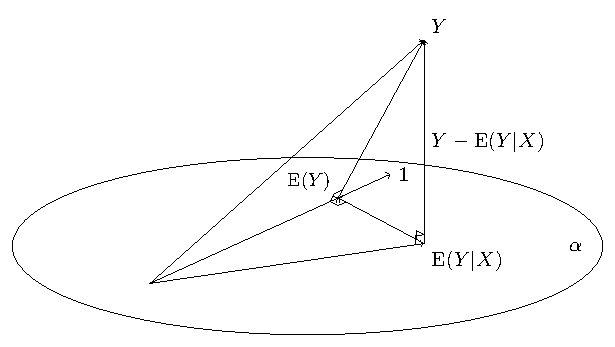
\includegraphics[width=0.6\linewidth]{figures/01_law_of_iterated_expectations.pdf}
\caption{The law of iterated expectations. Equivalence of the two-step projecttion
and direct projection of $Y$ onto $\mathbf{1}$.}
\label{fig:adams}
\end{center}
\end{figure}

\end{proof}


\subsection{MSE decomposition}

\begin{theorem}
The mean squared error of an estimator $\hat \theta$ with respect to an unknown
parameter $\theta$ defined as $MSE(\hat \theta) = \E((\hat \theta - \theta)^2)$
can be decomposed into the sum of the variance of the estimator and its squared bias:
\[
MSE(\hat \theta) = \Var(\hat \theta) + \E \left[\left( \E(\hat \theta) - \theta  \right)^2 \right]
\]
\end{theorem}

\marginnote{
\begin{align*}
&MSE(\hat \theta) = \E((\hat \theta - \theta)^2) \\
&= \E \left[ \left( \hat \theta - \E(\hat \theta) +  \E(\hat \theta) - \theta \right)^2 \right] \\
&= \E \left[ \left( \hat \theta - \E(\hat \theta) \right)^2 + 2  (\hat \theta - \E(\hat \theta)) (\E(\hat \theta) - \theta )  \right. \\
&+ \left. \left( \E(\hat \theta) - \theta  \right)^2 \right] \\
&= \E \left[\left( \hat \theta - \E(\hat \theta) \right)^2 \right] + 2 \E (\hat \theta - \E(\hat \theta)) (\E(\hat \theta) - \theta ) \\
&+ \E \left[\left( \E(\hat \theta) - \theta  \right)^2 \right] \\
&= \E \left[\left( \hat \theta - \E(\hat \theta) \right)^2 \right] \\
&+ 2 \E(\hat \theta - \E(\hat \theta)) \E(\hat \theta - \E(\hat \theta)) \\
&+ \E \left[\left( \E(\hat \theta) - \theta  \right)^2 \right] \\
&= \E \left[\left( \hat \theta - \E(\hat \theta) \right)^2 \right] + \E \left[\left( \E(\hat \theta) - \theta  \right)^2 \right] \\
&= \Var(\hat \theta) + \E \left[\left( \E(\hat \theta) - \theta  \right)^2 \right]
\end{align*}
}

\begin{proof}
We start with a random variable $\theta$ and its estimate $\hat \theta$ in the
vector space. We know that an unbiased estimator's projection would be exactly
the vector representing $\theta$. However, in general it does not have to and
Figure~\ref{fig:mse_decomposed} illustrates this case: the projection of the estimator falls onto
the line spanned by the vector $\theta$.

Connecting vectors $\theta$ and $\hat \theta$, we obtain the right triangle which
legs are $\hat \theta - \E(\hat\theta)$, $\E(\hat\theta) - \theta$ and the
hypotenuse $\hat \theta - \theta$.
Applying the Pythagorean theorem, we finish the proof:
\begin{align*}
\lVert \hat \theta - \theta \rVert^2 &= \lVert \hat \theta - \E(\hat \theta) \rVert^2  + \lVert \E(\hat \theta) - \theta \rVert^2 \\
\E((\hat \theta - \theta)^2) &= \E((\hat \theta - \E(\hat \theta))^2) + \E((\E(\hat \theta) - \theta)^2) \\
MSE(\hat \theta) &= \Var(\hat \theta) + \E((\E(\hat \theta) - \theta)^2)
\end{align*}

\begin{figure}[h!]
\begin{center}
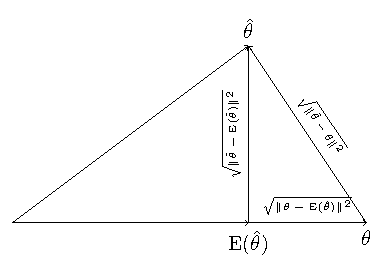
\includegraphics[width=0.6\linewidth]{figures/01_mse_decomposition.pdf}
\caption{Decomposition of mean squred error into the variance and the bias squared
$\left(a = \sqrt{\lVert\hat\theta - \E(\hat\theta)\rVert^2} \right.$, $b = \sqrt{\lVert \theta - \E(\hat\theta) \rVert^2}$, $\left. c = \sqrt{\lVert \hat\theta - \theta \rVert^2} \right)$}
\label{fig:mse_decomposed}
\setfloatalignment{b}
\end{center}
\end{figure}

\end{proof}
